% Options for packages loaded elsewhere
% Options for packages loaded elsewhere
\PassOptionsToPackage{unicode}{hyperref}
\PassOptionsToPackage{hyphens}{url}
\PassOptionsToPackage{dvipsnames,svgnames,x11names}{xcolor}
%
\documentclass[
  brazilian,
  authoryear,
  preprint]{elsarticle}
\usepackage{xcolor}
\usepackage{amsmath,amssymb}
\setcounter{secnumdepth}{5}
\usepackage{iftex}
\ifPDFTeX
  \usepackage[T1]{fontenc}
  \usepackage[utf8]{inputenc}
  \usepackage{textcomp} % provide euro and other symbols
\else % if luatex or xetex
  \usepackage{unicode-math} % this also loads fontspec
  \defaultfontfeatures{Scale=MatchLowercase}
  \defaultfontfeatures[\rmfamily]{Ligatures=TeX,Scale=1}
\fi
\usepackage{lmodern}
\ifPDFTeX\else
  % xetex/luatex font selection
\fi
% Use upquote if available, for straight quotes in verbatim environments
\IfFileExists{upquote.sty}{\usepackage{upquote}}{}
\IfFileExists{microtype.sty}{% use microtype if available
  \usepackage[]{microtype}
  \UseMicrotypeSet[protrusion]{basicmath} % disable protrusion for tt fonts
}{}
\makeatletter
\@ifundefined{KOMAClassName}{% if non-KOMA class
  \IfFileExists{parskip.sty}{%
    \usepackage{parskip}
  }{% else
    \setlength{\parindent}{0pt}
    \setlength{\parskip}{6pt plus 2pt minus 1pt}}
}{% if KOMA class
  \KOMAoptions{parskip=half}}
\makeatother
% Make \paragraph and \subparagraph free-standing
\makeatletter
\ifx\paragraph\undefined\else
  \let\oldparagraph\paragraph
  \renewcommand{\paragraph}{
    \@ifstar
      \xxxParagraphStar
      \xxxParagraphNoStar
  }
  \newcommand{\xxxParagraphStar}[1]{\oldparagraph*{#1}\mbox{}}
  \newcommand{\xxxParagraphNoStar}[1]{\oldparagraph{#1}\mbox{}}
\fi
\ifx\subparagraph\undefined\else
  \let\oldsubparagraph\subparagraph
  \renewcommand{\subparagraph}{
    \@ifstar
      \xxxSubParagraphStar
      \xxxSubParagraphNoStar
  }
  \newcommand{\xxxSubParagraphStar}[1]{\oldsubparagraph*{#1}\mbox{}}
  \newcommand{\xxxSubParagraphNoStar}[1]{\oldsubparagraph{#1}\mbox{}}
\fi
\makeatother


\usepackage{longtable,booktabs,array}
\usepackage{calc} % for calculating minipage widths
% Correct order of tables after \paragraph or \subparagraph
\usepackage{etoolbox}
\makeatletter
\patchcmd\longtable{\par}{\if@noskipsec\mbox{}\fi\par}{}{}
\makeatother
% Allow footnotes in longtable head/foot
\IfFileExists{footnotehyper.sty}{\usepackage{footnotehyper}}{\usepackage{footnote}}
\makesavenoteenv{longtable}
\usepackage{graphicx}
\makeatletter
\newsavebox\pandoc@box
\newcommand*\pandocbounded[1]{% scales image to fit in text height/width
  \sbox\pandoc@box{#1}%
  \Gscale@div\@tempa{\textheight}{\dimexpr\ht\pandoc@box+\dp\pandoc@box\relax}%
  \Gscale@div\@tempb{\linewidth}{\wd\pandoc@box}%
  \ifdim\@tempb\p@<\@tempa\p@\let\@tempa\@tempb\fi% select the smaller of both
  \ifdim\@tempa\p@<\p@\scalebox{\@tempa}{\usebox\pandoc@box}%
  \else\usebox{\pandoc@box}%
  \fi%
}
% Set default figure placement to htbp
\def\fps@figure{htbp}
\makeatother



\ifLuaTeX
\usepackage[bidi=basic]{babel}
\else
\usepackage[bidi=default]{babel}
\fi
% get rid of language-specific shorthands (see #6817):
\let\LanguageShortHands\languageshorthands
\def\languageshorthands#1{}


\setlength{\emergencystretch}{3em} % prevent overfull lines

\providecommand{\tightlist}{%
  \setlength{\itemsep}{0pt}\setlength{\parskip}{0pt}}



 
\usepackage[]{natbib}
\bibliographystyle{elsarticle-harv}


\usepackage{xcolor}
\makeatletter
\@ifpackageloaded{caption}{}{\usepackage{caption}}
\AtBeginDocument{%
\ifdefined\contentsname
  \renewcommand*\contentsname{Índice}
\else
  \newcommand\contentsname{Índice}
\fi
\ifdefined\listfigurename
  \renewcommand*\listfigurename{Lista de Figuras}
\else
  \newcommand\listfigurename{Lista de Figuras}
\fi
\ifdefined\listtablename
  \renewcommand*\listtablename{Lista de Tabelas}
\else
  \newcommand\listtablename{Lista de Tabelas}
\fi
\ifdefined\figurename
  \renewcommand*\figurename{Figura}
\else
  \newcommand\figurename{Figura}
\fi
\ifdefined\tablename
  \renewcommand*\tablename{Tabela}
\else
  \newcommand\tablename{Tabela}
\fi
}
\@ifpackageloaded{float}{}{\usepackage{float}}
\floatstyle{ruled}
\@ifundefined{c@chapter}{\newfloat{codelisting}{h}{lop}}{\newfloat{codelisting}{h}{lop}[chapter]}
\floatname{codelisting}{Listagem}
\newcommand*\listoflistings{\listof{codelisting}{Lista de Listagens}}
\makeatother
\makeatletter
\makeatother
\makeatletter
\@ifpackageloaded{caption}{}{\usepackage{caption}}
\@ifpackageloaded{subcaption}{}{\usepackage{subcaption}}
\makeatother
\journal{Catena}
\usepackage{bookmark}
\IfFileExists{xurl.sty}{\usepackage{xurl}}{} % add URL line breaks if available
\urlstyle{same}
\hypersetup{
  pdftitle={Impedância hidráulica, toxicidade por alumínio e vulnerabilidade geotécnica como amplificadores da erodibilidade efetiva em Plintossolos tropicais com erosão linear},
  pdfauthor={Emersson Guedes da Silva},
  pdflang={pt-BR},
  pdfkeywords={soil erodibility, USLE correction
factor, Plinthosol, Ferralsol, Acrisol, infiltration rate, aluminum
saturation, slope stability, tropical weathering},
  colorlinks=true,
  linkcolor={blue},
  filecolor={Maroon},
  citecolor={Blue},
  urlcolor={Blue},
  pdfcreator={LaTeX via pandoc}}


\setlength{\parindent}{6pt}
\begin{document}

\begin{frontmatter}
\title{Impedância hidráulica, toxicidade por alumínio e vulnerabilidade
geotécnica como amplificadores da erodibilidade efetiva em Plintossolos
tropicais com erosão linear}
\author[1]{Emersson Guedes da Silva%
\corref{cor1}%
}
 \ead{emersson.guedes@example.com} 

\affiliation[1]{organization={Universidade Federal de
Sergipe, Departamento de Zootecnia},city={São
Cristóvão},country={Brasil},countrysep={,},postcodesep={}}

\cortext[cor1]{Corresponding author}

        
\begin{abstract}
O fator de erodibilidade (\(K\)) da Equação Universal de Perdas de Solo
(USLE/RUSLE) é estimado por nomograma baseado em textura, matéria
orgânica, estrutura e permeabilidade, porém não incorpora a variação
espacial da velocidade de infiltração básica (VIB) ao longo da vertente,
a toxicidade por alumínio que suprime cobertura vegetal nem a
proximidade geotécnica ao colapso de taludes, condições que em
Plintossolos tropicais amplificam a erodibilidade efetiva de modo não
captado pelo nomograma de Wischmeier. Esta proposta fundamenta um fator
de correção multiplicativo (\(K_{plint}\)) composto por três termos
adimensionais (\(\alpha\), \(\beta\), \(\gamma\)) que representam,
respectivamente, a amplificação por regime hidráulico, a penalização por
toxicidade edáfica e a vulnerabilidade geotécnica à ruptura de taludes.
As formas funcionais foram derivadas dos dados de campo obtidos em
Plintossolo Argilúvico Distrófico nos Tabuleiros Costeiros de Sergipe
(VIB = 1,53--3,13 cm/h, saturação por alumínio m = 15--99\%, coesão c =
13,02 kPa, ângulo de atrito \(\phi\) = 34,93°, altura crítica \(H_c\) =
3,35 m). O desenho experimental é multi-classe, com 14 parcelas padrão
Wischmeier distribuídas em três sítios pedologicamente contrastantes
(Plintossolo como alvo de calibração, Latossolo Vermelho-Amarelo como
controle negativo e Argissolo Vermelho-Amarelo como controle parcial),
de modo a isolar a contribuição de cada termo de correção e testar a
especificidade pedológica do fator proposto. A replicação temporal ao
longo de dois anos hidrológicos compensa o número reduzido de parcelas,
gerando centenas de observações independentes de \(K_{obs}\) por sítio.
A viabilidade matemática e a consistência física da formulação foram
previamente validadas por cinco testes computacionais (calibração
sintética, sensibilidade de Sobol, estabilidade de taludes, infiltração
Green-Ampt e erosão virtual) descritos em manuscrito complementar.
Apresentam-se as hipóteses, o protocolo de ensaios por classe de solo, a
estratégia de calibração sequencial e a validação cruzada entre sítios.
\end{abstract}





\begin{keyword}
    soil erodibility \sep USLE correction
factor \sep Plinthosol \sep Ferralsol \sep Acrisol \sep infiltration
rate \sep aluminum saturation \sep slope stability \sep 
    tropical weathering
\end{keyword}
\end{frontmatter}
    

\section{1. Introdução}\label{introduuxe7uxe3o}

A erosão hídrica acelerada constitui uma das principais ameaças à
sustentabilidade de solos tropicais, com taxas de perda de solo que
excedem a pedogênese natural em ordens de grandeza nas vertentes mais
vulneráveis \citep{poesen_2018}. A Equação Universal de Perdas de Solo
(USLE), na formulação original de \citet{wischmeier_smith_1978} e na
revisão RUSLE de \citet{renard_et_al_1997}, permanece como o modelo
empírico mais adotado globalmente para estimativa de erosão laminar e em
sulcos, estruturando a perda de solo como produto de seis fatores que
descrevem erosividade da chuva, erodibilidade do solo, comprimento e
declividade da rampa, cobertura vegetal e práticas conservacionistas.

O fator de erodibilidade (\(K\)) sintetiza a suscetibilidade intrínseca
do solo ao destacamento e transporte por impacto de gotas e escoamento
laminar. Sua estimativa pelo nomograma de \citet{wischmeier_et_al_1971}
depende de cinco propriedades do horizonte superficial, notadamente
granulometria, matéria orgânica, estrutura e permeabilidade, e foi
calibrada em parcelas experimentais de solos temperados do Meio-Oeste
dos Estados Unidos, em condições edáficas e climáticas distintas dos
trópicos úmidos \citep{alewell_et_al_2019}. A aplicação desse nomograma
a solos tropicais intemperizados enfrenta limitações reconhecidas na
literatura. Solos com elevada fração argilosa (\textgreater{} 40\%) mas
com argilas 1:1 (caulinita) e oxi-hidróxidos de ferro e alumínio
apresentam microagregação estável que reduz a erodibilidade efetiva em
relação ao previsto pela granulometria
\citep{silva_et_al_2009, bertoni_lombardi_neto_2017}, ao passo que em
Plintossolos com impedância hidráulica em subsuperfície a erodibilidade
efetiva pode superar a prevista porque a geração de escoamento
concentrado sob intensidades de chuva recorrentes amplifica o
destacamento em magnitudes que a equação empírica não prevê
\citep{poesen_2018, cassol_et_al_2023}.

Essa discrepância é particularmente aguda quando a erosão transcende o
domínio laminar e em sulcos para o qual a USLE foi calibrada. Em
vertentes com ravinas ativas, a perda de solo integra contribuições de
incisão vertical, colapso de taludes e recuo de cabeceira, processos
governados por tensão cisalhante do escoamento concentrado e por
resistência geotécnica do substrato (coesão, ângulo de atrito, pressões
neutras) que o fator \(K\) não contempla
\citep{poesen_et_al_2003, liu_et_al_2021}. Modelos como EGEM, WEPP e
SWAT tratam erosão em ravinas como processo separado, porém sua
complexidade computacional e demanda de dados limitam a adoção em
contextos operacionais de planejamento \citep{alewell_et_al_2019}.

Em Plintossolos tropicais, três condições edáficas convergem para
amplificar a erodibilidade efetiva de modo não captado pelo nomograma. A
impedância hidráulica imposta pela presença de plintita em subsuperfície
reduz drasticamente a velocidade de infiltração básica (VIB),
convertendo o regime de percolação vertical predominante em escoamento
hortoniano a partir de intensidades de chuva relativamente modestas. A
saturação por alumínio elevada nos horizontes subsuperficiais
(frequentemente superior a 80\%) restringe a colonização radicular e
suprime a cobertura vegetal, expondo o horizonte a destacamento direto e
retroalimentando a amplificação da erodibilidade, processo cíclico
documentado em solos álicos tropicais \citep{cassol_et_al_2023}. A
proximidade geotécnica ao limiar de ruptura por cisalhamento, expressa
pela razão entre profundidade da feição e altura crítica de Rankine
(\(H/H_c\)), introduz contribuição de colapso de taludes que cresce de
modo não linear à medida que a feição se aprofunda
\citep{poesen_et_al_2003, sidorchuk_2006}.

Em trabalho anterior conduzido nos Tabuleiros Costeiros de Sergipe,
caracterizou-se um Plintossolo Argilúvico Distrófico com VIB de 1,53
cm/h nos terços intermediário e inferior da vertente, saturação por
alumínio de 84--99\% nos horizontes subsuperficiais, coesão sob
saturação de 13,02 kPa e ângulo de atrito de 34,93° (horizonte Bt, 1,20
m), resultando em altura crítica de corte vertical \(H_c\) = 3,35 m.
Seis feições erosivas com profundidade de 0,40--1,50 m e razão \(H/H_c\)
de 0,12--0,45 foram classificadas por inferência fuzzy Mamdani como
ravinas transicionais a voçorocas incipientes. Esses dados sugerem que a
convergência das três condições amplificadoras eleva a erodibilidade
efetiva do Plintossolo acima do previsto pelo nomograma, motivando a
proposição de um fator de correção específico.

A confirmação de que essa amplificação é atribuível às propriedades
diagnósticas do Plintossolo, e não a um artefato generalizável a
qualquer solo tropical intemperizado, requer confrontação com classes
pedológicas contrastantes. Latossolos Vermelho-Amarelos da mesma região
apresentam VIB tipicamente superior a 6 cm/h, saturação por alumínio
inferior a 30\% e feições erosivas lineares ausentes ou incipientes,
constituindo controle negativo no qual se espera erodibilidade observada
próxima à prevista pelo nomograma
\citep{silva_et_al_2009, bertoni_lombardi_neto_2017}. Argissolos
Vermelho-Amarelos, por sua vez, compartilham com o Plintossolo o
gradiente textural abrupto (horizonte Bt adensado) que gera impedância
hidráulica e redução da VIB, porém sem plintita e frequentemente com
saturação por alumínio intermediária, operando como controle parcial que
permite isolar o efeito do regime hidráulico das demais amplificações.

Até o presente momento, nenhum estudo propôs um fator de correção para o
\(K\) da USLE/RUSLE que incorpore simultaneamente impedância hidráulica
subsuperficial, toxicidade edáfica por alumínio e vulnerabilidade
geotécnica ao colapso de taludes, nem validou tal formulação por
confrontação multi-classe entre solos tropicais com gradientes
contrastantes dessas propriedades.

Este estudo propõe a fundamentação teórica e o desenho experimental
multi-classe para calibração de um fator de correção multiplicativo
(\(K_{plint}\)) que incorpora regime hidráulico, toxicidade edáfica e
vulnerabilidade geotécnica ao fator \(K\) da USLE/RUSLE, utilizando
Plintossolo como alvo de calibração, Latossolo como controle negativo e
Argissolo como controle parcial. A viabilidade matemática
(identificabilidade paramétrica, sensibilidade e consistência física) da
formulação proposta foi previamente avaliada por cinco testes
computacionais apresentados em manuscrito complementar, cujos resultados
sustentam a adequação do desenho experimental aqui descrito.

\section{2. Fundamentação teórica}\label{fundamentauxe7uxe3o-teuxf3rica}

\subsection{2.1 A USLE e o nomograma de
erodibilidade}\label{a-usle-e-o-nomograma-de-erodibilidade}

A perda de solo média anual pela USLE é expressa como produto de seis
fatores (Equação~\ref{eq-usle}).

\begin{equation}\phantomsection\label{eq-usle}{
A = R \times K \times L \times S \times C \times P
}\end{equation}

onde \(A\) é a perda de solo média anual (t ha\(^{-1}\) ano\(^{-1}\)),
\(R\) o fator de erosividade da chuva (MJ mm ha\(^{-1}\) h\(^{-1}\)
ano\(^{-1}\)), \(K\) o fator de erodibilidade do solo (t h MJ\(^{-1}\)
mm\(^{-1}\)), \(L\) o fator de comprimento de rampa, \(S\) o fator de
declividade, \(C\) o fator de cobertura e manejo e \(P\) o fator de
práticas conservacionistas. O fator \(K\) é estimado pela equação do
nomograma (Equação~\ref{eq-nomograma}).

\begin{equation}\phantomsection\label{eq-nomograma}{
100\,K = 2{,}1 \times 10^{-4}\,M^{1{,}14}\,(12 - a) + 3{,}25\,(b - 2) + 2{,}5\,(c - 3)
}\end{equation}

onde
\(M = (\%\text{silte} + \%\text{areia muito fina}) \times (100 - \%\text{argila})\),
\(a\) é o teor de matéria orgânica (\%), \(b\) o código de estrutura do
solo (1--4) e \(c\) o código de permeabilidade (1--6).

\subsection{\texorpdfstring{2.2 Estrutura do fator de correção
\(K_{plint}\)}{2.2 Estrutura do fator de correção K\_\{plint\}}}\label{estrutura-do-fator-de-correuxe7uxe3o-k_plint}

A erodibilidade corrigida para Plintossolos tropicais com erosão linear
é expressa como produto do fator \(K\) do nomograma de Wischmeier por
três termos de correção adimensionais (Equação~\ref{eq-kplint}).

\begin{equation}\phantomsection\label{eq-kplint}{
K_{plint} = K_{RUSLE} \times \alpha(VIB) \times \beta(m_{Al}) \times \gamma\!\left(\dfrac{H}{H_c}\right)
}\end{equation}

onde \(K_{RUSLE}\) é o fator de erodibilidade obtido pela
Equação~\ref{eq-nomograma} ou por medição direta em parcela padrão,
\(\alpha\) o fator de amplificação por regime hidráulico, \(\beta\) o
fator de penalização por toxicidade edáfica e \(\gamma\) o fator de
vulnerabilidade geotécnica. A estrutura multiplicativa implica que cada
fator opera como amplificador independente.

Quando nenhuma das três condições amplificadoras está presente (solo bem
drenado, ausência de toxicidade por alumínio, ausência de feição erosiva
profunda), os três fatores assumem valor unitário e \(K_{plint}\) se
reduz a \(K_{RUSLE}\). Quando as três condições convergem, como em
Plintossolos com voçorocas ativas, os fatores se multiplicam e a razão
\(\delta = K_{plint}/K_{RUSLE} = \alpha \times \beta \times \gamma\)
pode atingir valores de 2 a 10 ou superiores \citep{poesen_2018}. A
variável \(\delta\) é adimensional e independente do valor absoluto de
\(K_{RUSLE}\), permitindo comparar o grau de amplificação entre classes
pedológicas com erodibilidade basal distinta.

\subsection{\texorpdfstring{2.3 Fator de amplificação por regime
hidráulico
\(\alpha(VIB)\)}{2.3 Fator de amplificação por regime hidráulico \textbackslash alpha(VIB)}}\label{fator-de-amplificauxe7uxe3o-por-regime-hidruxe1ulico-alphavib}

O nomograma de Wischmeier atribui à permeabilidade um peso relativamente
baixo no cômputo de \(K\) (código 1--6, contribuição máxima de 7,5\% no
valor final). Em solos com boa drenagem interna, a maior parte da
precipitação infiltra e percola verticalmente, gerando pouco escoamento
superficial e, consequentemente, baixa energia disponível para
destacamento e transporte de partículas \citep{deroo_1992}. Em
Plintossolos, horizontes subsuperficiais com plintita ou petroplintita
apresentam condutividade hidráulica saturada muito inferior à dos
horizontes sobrejacentes, criando barreira à percolação que favorece a
saturação do perfil e o escoamento hortoniano por excesso de saturação
\citep{padmanabhan_2005}. A VIB, determinada em campo por infiltrômetro
de duplo anel, reflete essa impedância integrada ao longo do perfil e
constitui a variável de entrada mais acessível para expressar o
contraste hidrológico entre classes de solo
\citep{bertoni_lombardi_neto_2017}.

No Plintossolo estudado, a VIB varia de 3,13 cm/h no terço superior a
1,53 cm/h no intermediário (redução de 51\%), transição que converte o
regime de percolação vertical predominante em escoamento hortoniano e
amplifica a energia erosiva efetiva de modo desproporcional ao previsto
pelo código de permeabilidade do nomograma \citep{poesen_2018}.

A forma funcional proposta para \(\alpha\) é uma lei de potência
referenciada a um limiar de VIB acima do qual o perfil opera
predominantemente sob regime de percolação vertical e a contribuição da
impedância hidráulica à erodibilidade é negligenciável
(Equação~\ref{eq-alpha}).

\begin{equation}\phantomsection\label{eq-alpha}{
\alpha(VIB) = \left(\dfrac{VIB_{ref}}{VIB_{local}}\right)^{n_1}
}\end{equation}

onde \(VIB_{ref}\) é o limiar de referência (cm/h) acima do qual o
perfil opera sob percolação vertical predominante e \(n_1\) o expoente
de amplificação a calibrar. O expoente \(n_1\) governa a intensidade da
penalização à medida que a VIB decresce, de modo que para \(n_1 = 1\) a
relação é linear e reduzir a VIB pela metade duplica \(\alpha\),
enquanto valores de \(n_1 > 1\) produzem penalização mais severa em
solos com impedância acentuada e \(n_1 < 1\) atenua a diferenciação
entre solos com VIB moderada e muito baixa \citep{kinnell_2005}. O
limiar \(VIB_{ref}\) = 6,0 cm/h corresponde ao limite inferior de solos
classificados como bem drenados na pedologia tropical
\citep{embrapa_2018} e foi adotado como ponto de neutralidade
(\(\alpha = 1\)) do fator hidráulico.

Esse valor foi corroborado empiricamente pela classificação fuzzy de
severidade desenvolvida para o sítio, na qual feições situadas acima
desse patamar não atingem severidade transicional mesmo com
profundidades de 2 m.

Para \(VIB_{local} \geq VIB_{ref}\), adota-se \(\alpha = 1\) (sem
correção). Para \(VIB_{local} < VIB_{ref}\), \(\alpha > 1\) com
magnitude crescente conforme o inverso da infiltração. No Plintossolo
estudado, a VIB do horizonte intermediário (BAc) é 1,53 cm/h, resultando
em \(\alpha = (6{,}0/1{,}53)^{n_1} = 3{,}92^{n_1}\), o que para
\(n_1 = 1\) indica que a impedância hidráulica subsuperficial amplifica
a erodibilidade efetiva em quase quatro vezes em relação a um solo com
VIB de referência. Um Latossolo Vermelho-Amarelo típico com VIB de 9
cm/h apresenta \(\alpha = 1\) (\(VIB > VIB_{ref}\)), ilustrando a
capacidade do fator de distinguir classes bem drenadas de classes com
impedância hidráulica sem modelagem hidrológica detalhada. Os valores de
\(\alpha\) para três posições da vertente e cenários de \(n_1\) são
apresentados na Tabela 1.

Tabela 1. Valores de \(\alpha\) para três posições da vertente em função
de \(n_1\) hipotético

\begin{longtable}[]{@{}
  >{\raggedright\arraybackslash}p{(\linewidth - 8\tabcolsep) * \real{0.1579}}
  >{\raggedleft\arraybackslash}p{(\linewidth - 8\tabcolsep) * \real{0.2105}}
  >{\raggedleft\arraybackslash}p{(\linewidth - 8\tabcolsep) * \real{0.2105}}
  >{\raggedleft\arraybackslash}p{(\linewidth - 8\tabcolsep) * \real{0.2105}}
  >{\raggedleft\arraybackslash}p{(\linewidth - 8\tabcolsep) * \real{0.2105}}@{}}
\toprule\noalign{}
\begin{minipage}[b]{\linewidth}\raggedright
Posição
\end{minipage} & \begin{minipage}[b]{\linewidth}\raggedleft
VIB (cm/h)
\end{minipage} & \begin{minipage}[b]{\linewidth}\raggedleft
\(\alpha\) (\(n_1\) = 0,5)
\end{minipage} & \begin{minipage}[b]{\linewidth}\raggedleft
\(\alpha\) (\(n_1\) = 1,0)
\end{minipage} & \begin{minipage}[b]{\linewidth}\raggedleft
\(\alpha\) (\(n_1\) = 1,5)
\end{minipage} \\
\midrule\noalign{}
\endhead
\bottomrule\noalign{}
\endlastfoot
Terço superior & 3,13 & 1,38 & 1,92 & 2,66 \\
Terço intermediário & 1,53 & 1,98 & 3,92 & 7,76 \\
Terço inferior & 1,59 & 1,94 & 3,77 & 7,33 \\
\end{longtable}

\subsection{\texorpdfstring{2.4 Fator de penalização por toxicidade
edáfica
\(\beta(m_{Al})\)}{2.4 Fator de penalização por toxicidade edáfica \textbackslash beta(m\_\{Al\})}}\label{fator-de-penalizauxe7uxe3o-por-toxicidade-eduxe1fica-betam_al}

A saturação por alumínio (\(m\)) nos horizontes subsuperficiais do
Plintossolo estudado varia de 15,2\% no Ap a 99,2\% no BAc, constituindo
gradiente de toxicidade que restringe progressivamente a colonização
radicular e a cobertura vegetal \citep{de_oliveira_et_al_2024}.

Embora o fator \(C\) da USLE capture parcialmente o efeito da cobertura,
ele não incorpora o mecanismo causal edáfico que a determina nem a
retroalimentação entre perda de cobertura, exposição do horizonte e
amplificação da erodibilidade, processo cíclico documentado em solos
álicos tropicais \citep{cassol_et_al_2023}.

A forma funcional proposta é uma sigmoide logística com inflexão no
limiar de caráter álico (Equação~\ref{eq-beta}).

\begin{equation}\phantomsection\label{eq-beta}{
\beta(m) = 1 + \dfrac{\beta_{max} - 1}{1 + \exp\!\left[-k_2\,(m - m_0)\right]}
}\end{equation}

onde \(m\) é a saturação por alumínio do horizonte diagnóstico (\%,
0--100), \(m_0\) o ponto de inflexão coincidente com o limiar
convencional de caráter álico (\%), \(k_2\) o parâmetro de inclinação da
sigmoide (adimensional) e \(\beta_{max}\) o fator máximo de
amplificação. Para \(m_{Al}\) muito abaixo de \(m_0\), o denominador é
grande e \(\beta\) se aproxima de 1, indicando que a fitotoxicidade é
insuficiente para suprimir mensuravelmente a vegetação. Para \(m_{Al}\)
muito acima de \(m_0\), a função converge para \(\beta_{max}\),
representando a amplificação máxima atribuível exclusivamente à
toxicidade. O parâmetro \(k_2\) controla a abruptidade da transição, com
valores altos produzindo mudança rápida em torno de 50\% e valores
baixos gerando gradiente suave ao longo de toda a faixa de saturação.

Com base na literatura de fitotoxicidade por alumínio em solos
tropicais, propõe-se \(m_0\) = 50\% como ponto de inflexão, valor acima
do qual a maioria das gramíneas forrageiras tropicais apresenta redução
de cobertura superior a 50\% \citep{embrapa_2018}. Os parâmetros \(k_2\)
e \(\beta_{max}\) constituem os termos a calibrar experimentalmente.
Para o Plintossolo estudado, considerando valores preliminares de
\(\beta_{max} = 2{,}5\) e \(k_2 = 0{,}10\), o horizonte Ap (\(m\) =
15,2\%) resulta em \(\beta \approx 1{,}04\), praticamente sem
amplificação, enquanto o horizonte BAc (\(m\) = 99,2\%) atinge
\(\beta \approx 2{,}47\), próximo ao máximo.

Agronomicamente, esse gradiente vertical indica que a superfície do solo
ainda pode sustentar cobertura vegetal esparsa, porém os horizontes
subsuperficiais expostos nos taludes das feições erosivas estão
desprovidos de proteção radicular contra o desprendimento por escoamento
concentrado \citep{vannoppen_2015}. A sigmoide captura essa não
linearidade com apenas dois parâmetros livres (\(\beta_{max}\) e
\(k_2\)).

\subsection{\texorpdfstring{2.5 Fator de vulnerabilidade geotécnica
\(\gamma(H/H_c)\)}{2.5 Fator de vulnerabilidade geotécnica \textbackslash gamma(H/H\_c)}}\label{fator-de-vulnerabilidade-geotuxe9cnica-gammahh_c}

A USLE foi concebida para erosão laminar e em sulcos, processos
governados por destacamento superficial por impacto de gotas (splash) e
tensão cisalhante de escoamento raso. Em vertentes com feições erosivas
que se aprofundam em direção à altura crítica de ruptura por
cisalhamento (\(H_c\)), a contribuição de movimentos de massa nas
paredes das feições (escorregamentos translacionais e rotacionais) à
perda total de solo cresce de modo não linear, processo que o fator
\(K\) não contempla \citep{poesen_et_al_2003, sidorchuk_2006}.

A razão \(H/H_c\) (profundidade máxima da feição dividida pela altura
crítica de Rankine) constitui indicador adimensional normalizado da
proximidade ao limiar de ruptura. Para \(H/H_c \to 0\) (sulcos rasos), a
contribuição geotécnica é desprezível; para \(H/H_c \to 1\), o talude
opera próximo ao equilíbrio limite e episódios de saturação sazonal com
desenvolvimento de poropressões positivas podem disparar escorregamentos
translacionais e mobilização volumétrica de solo, amplificando a perda
de solo em ordens de grandeza superiores ao previsto pela USLE.

A forma funcional proposta é uma função de potência com origem unitária
(Equação~\ref{eq-gamma}).

\begin{equation}\phantomsection\label{eq-gamma}{
\gamma\!\left(\dfrac{H}{H_c}\right) = 1 + k_3 \cdot \left(\dfrac{H}{H_c}\right)^{n_3}
}\end{equation}

onde \(H\) é a profundidade máxima da feição (m), \(H_c\) a altura
crítica de corte vertical sob saturação (m), \(k_3\) o coeficiente de
escala da amplificação geotécnica e \(n_3\) o expoente de curvatura da
resposta. Para \(H/H_c = 0\), \(\gamma = 1\) (sem contribuição
geotécnica).

Valores elevados de \(n_3\) (\textgreater{} 2) fazem com que \(\gamma\)
permaneça próximo de 1 para feições rasas e aumente abruptamente apenas
quando \(H/H_c\) se aproxima de 1, comportamento fisicamente coerente
porque o volume de solo mobilizado pela cunha de ruptura cresce com
potência cúbica ou superior da altura da parede. A escolha de
\(n_3 = 2\) como valor inicial é motivada pela dependência quadrática
entre volume mobilizado por colapso e altura de queda em modelos de
ruptura planar \citep{fredlund_rahardjo_1993}.

A altura crítica \(H_c\) é estimada pela teoria de Rankine para corte
vertical com fissura de tração preenchida por água
(Equação~\ref{eq-hc}).

\begin{equation}\phantomsection\label{eq-hc}{
H_c = \dfrac{2\,c}{\gamma_{sat}} \cdot \tan\!\left(45° + \dfrac{\phi}{2}\right) + \dfrac{2\,c}{\gamma_{sat} \cdot \tan\!\left(45° + \dfrac{\phi}{2}\right)}
}\end{equation}

onde \(c\) é a coesão efetiva sob saturação (kPa), \(\phi\) o ângulo de
atrito interno (°) e \(\gamma_{sat}\) o peso específico saturado do solo
(kN/m³). A formulação assume análise em tensões totais com pressão
neutra nula (\(u = 0\)), consistente com a determinação de \(c\) e
\(\phi\) por ensaio de cisalhamento direto em amostras saturadas (ASTM
D3080).

A influência de poropressões positivas sob condições de campo é avaliada
separadamente na análise de estabilidade de taludes apresentada no
manuscrito complementar. Para o Plintossolo estudado (\(c\) = 13,02 kPa,
\(\phi\) = 34,93°, \(\gamma_{sat}\) = 19,93 kN/m³), \(H_c\) = 3,35 m.

Os valores de \(\gamma\) para as seis feições inventariadas são
apresentados na Tabela 2 para cenários de \(k_3\) e \(n_3\).

Tabela 2. Valores de \(\gamma\) para as seis feições erosivas em função
de \(k_3\) e \(n_3\) hipotéticos

\begin{longtable}[]{@{}
  >{\centering\arraybackslash}p{(\linewidth - 10\tabcolsep) * \real{0.2000}}
  >{\raggedleft\arraybackslash}p{(\linewidth - 10\tabcolsep) * \real{0.1600}}
  >{\raggedleft\arraybackslash}p{(\linewidth - 10\tabcolsep) * \real{0.1600}}
  >{\raggedleft\arraybackslash}p{(\linewidth - 10\tabcolsep) * \real{0.1600}}
  >{\raggedleft\arraybackslash}p{(\linewidth - 10\tabcolsep) * \real{0.1600}}
  >{\raggedleft\arraybackslash}p{(\linewidth - 10\tabcolsep) * \real{0.1600}}@{}}
\toprule\noalign{}
\begin{minipage}[b]{\linewidth}\centering
Feição
\end{minipage} & \begin{minipage}[b]{\linewidth}\raggedleft
Prof.~(m)
\end{minipage} & \begin{minipage}[b]{\linewidth}\raggedleft
\(H/H_c\)
\end{minipage} & \begin{minipage}[b]{\linewidth}\raggedleft
\(\gamma\) (\(k_3\)=2, \(n_3\)=2)
\end{minipage} & \begin{minipage}[b]{\linewidth}\raggedleft
\(\gamma\) (\(k_3\)=5, \(n_3\)=2)
\end{minipage} & \begin{minipage}[b]{\linewidth}\raggedleft
\(\gamma\) (\(k_3\)=2, \(n_3\)=3)
\end{minipage} \\
\midrule\noalign{}
\endhead
\bottomrule\noalign{}
\endlastfoot
F1 & 1,10 & 0,33 & 1,22 & 1,54 & 1,07 \\
F2 & 0,40 & 0,12 & 1,03 & 1,07 & 1,00 \\
F3 & 0,60 & 0,18 & 1,06 & 1,16 & 1,01 \\
F4 & 1,40 & 0,42 & 1,35 & 1,88 & 1,15 \\
F5 & 1,50 & 0,45 & 1,40 & 2,01 & 1,18 \\
F6 & 0,60 & 0,18 & 1,06 & 1,16 & 1,01 \\
\end{longtable}

As seis feições mapeadas apresentam profundidades de 0,40 a 1,50 m
(\(H/H_c = 0{,}12\) a 0,45), intervalo no qual \(\gamma\) permanece
próximo de 1 e o colapso geotécnico não é o mecanismo dominante de perda
de solo. Em voçorocas regionais com profundidade superior a 2 m
(\(H/H_c > 0{,}6\)), contudo, \(\gamma\) pode contribuir
substancialmente para a amplificação total, o que justifica a inclusão
desse termo no modelo.

A adoção da teoria de Rankine para cortes verticais é uma simplificação
conservadora; para geometrias de talude com inclinação inferior a 90°,
métodos de equilíbrio limite como Bishop simplificado podem fornecer
valores de fator de segurança menos conservadores
\citep{fredlund_rahardjo_1993}, aspecto que requer verificação em
trabalho complementar.

\subsection{\texorpdfstring{2.6 Expressão expandida do
\(K_{plint}\)}{2.6 Expressão expandida do K\_\{plint\}}}\label{expressuxe3o-expandida-do-k_plint}

A substituição das Equação~\ref{eq-alpha}, Equação~\ref{eq-beta} e
Equação~\ref{eq-gamma} na Equação~\ref{eq-kplint} produz a expressão
completa (Equação~\ref{eq-kplint-exp}).

\begin{equation}\phantomsection\label{eq-kplint-exp}{
K_{plint} = K_{RUSLE} \times \left(\dfrac{VIB_{ref}}{VIB_{local}}\right)^{n_1} \times \left[1 + \dfrac{\beta_{max} - 1}{1 + e^{-k_2(m - m_0)}}\right] \times \left[1 + k_3 \cdot \left(\dfrac{H}{H_c}\right)^{n_3}\right]
}\end{equation}

A Equação~\ref{eq-kplint-exp} contém cinco parâmetros livres (\(n_1\),
\(\beta_{max}\), \(k_2\), \(k_3\), \(n_3\)) a serem estimados por
calibração em campo, e dois parâmetros fixados a priori (\(VIB_{ref}\) =
6 cm/h e \(m_0\) = 50\%) derivados de evidências pedológicas e limiares
de fitotoxicidade documentados em solos tropicais \citep{embrapa_2018}.
A razão
\(\delta = K_{plint}/K_{RUSLE} = \alpha \times \beta \times \gamma\)
sintetiza a amplificação total da erodibilidade e constitui a
variável-resposta da validação computacional e experimental. A
calibração requer, no mínimo, estimativas independentes de \(K_{obs}\)
em posições da vertente com variação simultânea de VIB, \(m\) e
\(H/H_c\), conforme descrito na seção 4.

\section{3. Hipóteses}\label{hipuxf3teses}

A estrutura multiplicativa da Equação~\ref{eq-kplint-exp} gera cinco
predições testáveis, cada uma vinculada a um dos termos do modelo ou à
sua interação.

A primeira hipótese (H1, regime hidráulico) prediz que a erodibilidade
observada (\(K_{obs}\)) no terço intermediário da vertente (VIB = 1,53
cm/h) é significativamente maior do que a prevista pelo nomograma
(\(K_{RUSLE}\)), com razão \(K_{obs}/K_{RUSLE} > 2{,}0\), ao passo que
no terço superior (VIB = 3,13 cm/h) essa razão tende à unidade. A
segunda hipótese (H2, toxicidade edáfica) prediz que, controlando-se VIB
e declividade, parcelas com horizonte diagnóstico exposto com saturação
por alumínio superior a 80\% apresentam \(K_{obs}\) pelo menos 1,5 vezes
superior ao de parcelas com saturação inferior a 50\%, refletindo o
efeito da supressão de cobertura vegetal sobre a erodibilidade.

A terceira hipótese (H3, vulnerabilidade geotécnica) estabelece que
parcelas adjacentes a feições com \(H/H_c > 0{,}40\) (F4, F5) produzem
perda de solo total (laminar e colapso de talude combinados)
significativamente maior do que parcelas adjacentes a feições com
\(H/H_c < 0{,}20\) (F2, F3), em proporção que excede a diferença
prevista pela USLE convencional. A quarta hipótese (H4, interação
multiplicativa) testa se o modelo da Equação~\ref{eq-kplint-exp} explica
proporção significativamente maior da variância de \(K_{obs}\) do que
modelos aditivos (\(K_{RUSLE} + \alpha + \beta + \gamma\)) ou do que
\(K_{RUSLE}\) isoladamente, avaliada por \(R^2\) ajustado e critério de
informação de Akaike.

A quinta hipótese (H5, especificidade pedológica) prediz que a
discrepância \(\delta = K_{obs}/K_{RUSLE}\) segue a hierarquia
\(\delta_{Plintossolo} > \delta_{Argissolo} > \delta_{Latossolo} \approx 1{,}0\),
confirmando que a amplificação é atribuível à convergência das condições
diagnósticas do Plintossolo (impedância hidráulica, toxicidade extrema e
proximidade geotécnica) e não a um artefato generalizado de solos
tropicais intemperizados. Essa hierarquia já foi corroborada
computacionalmente pela validação apresentada no Artigo 2, no qual o
Latossolo virtual apresentou \(\delta\) mediano de 1,04--1,07 em todas
as realizações.

\section{4. Desenho experimental}\label{desenho-experimental}

\subsection{4.1 Área de estudo e dados de
entrada}\label{uxe1rea-de-estudo-e-dados-de-entrada}

O sítio experimental está localizado na unidade geomorfológica dos
Tabuleiros Costeiros do estado de Sergipe, Nordeste do Brasil, sobre um
Plintossolo Háplico desenvolvido a partir de sedimentos do Grupo
Barreiras \citep{nascimento_pedrotti_2004}. O clima é tropical úmido (As
na classificação de Köppen), com precipitação média anual de 1200 a 1400
mm concentrada entre abril e agosto e temperatura média de 25 °C.

O uso predominante da terra é pastagem degradada com cobertura esparsa,
condição que expõe os horizontes subsuperficiais à ação direta do
escoamento concentrado. O sítio ocupa um interflúvio suavemente ondulado
onde a combinação de vegetação esparsa e plintita subsuperficial
favoreceu o desenvolvimento de múltiplas feições de erosão linear ao
longo do eixo de drenagem (Fig. Figura~\ref{fig-area-aerea}).

\begin{figure}

\centering{

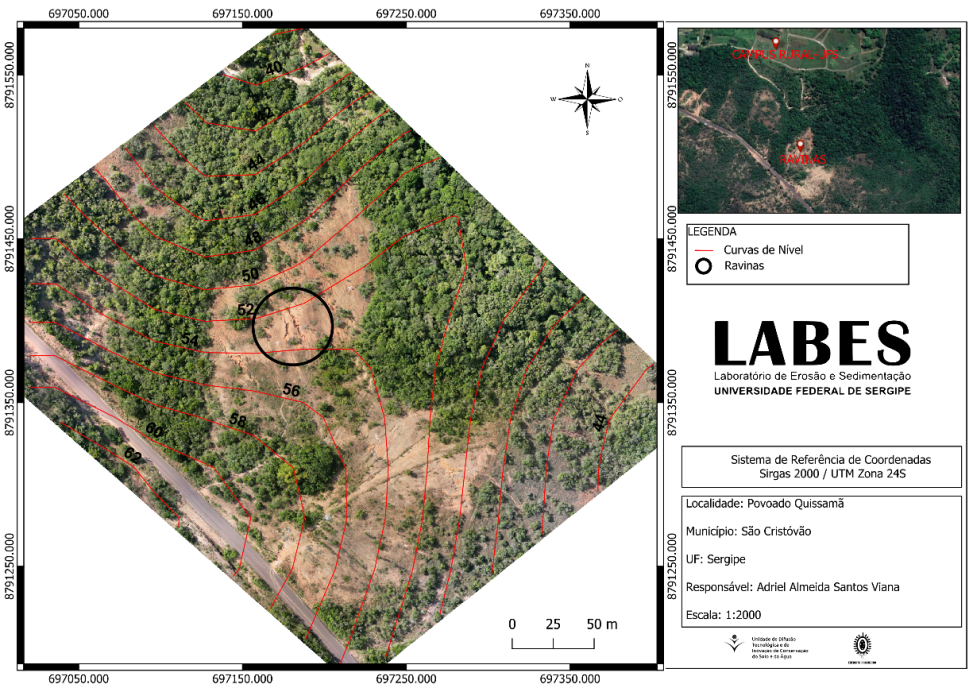
\includegraphics[width=0.9\linewidth,height=\textheight,keepaspectratio]{figuras/fig_00a_area_estudo_aerea.png}

}

\caption{\label{fig-area-aerea}Vista aérea mostrando a paisagem de
pastagem degradada e a ocorrência de feições de erosão linear no
Plintossolo Háplico dos Tabuleiros Costeiros de Sergipe, Nordeste do
Brasil.}

\end{figure}%

Seis feições erosivas ativas (F1 a F6) foram identificadas a partir de
ortomosaicos derivados de VANT com densidade média de nuvem de pontos de
120 pontos/m², e seus parâmetros morfométricos (profundidade, largura e
comprimento) validados por medições diretas em campo com trena (Fig.
Figura~\ref{fig-feicoes-campo}). As profundidades das feições variaram
de 0,40 m (F2) a 1,50 m (F5), correspondendo a profundidades
normalizadas \(H/H_c\) de 0,12 a 0,45 em relação à altura crítica
\(H_c = 3{,}35\) m calculada a partir dos parâmetros geotécnicos medidos
em campo via Equação~\ref{eq-hc}. Esse intervalo indica que o colapso
lateral de talude ainda não se tornou o mecanismo dominante de perda de
solo em nenhuma das feições levantadas, condição que restringe a faixa
de calibração do fator geotécnico \(\gamma\).

\begin{figure}

\centering{

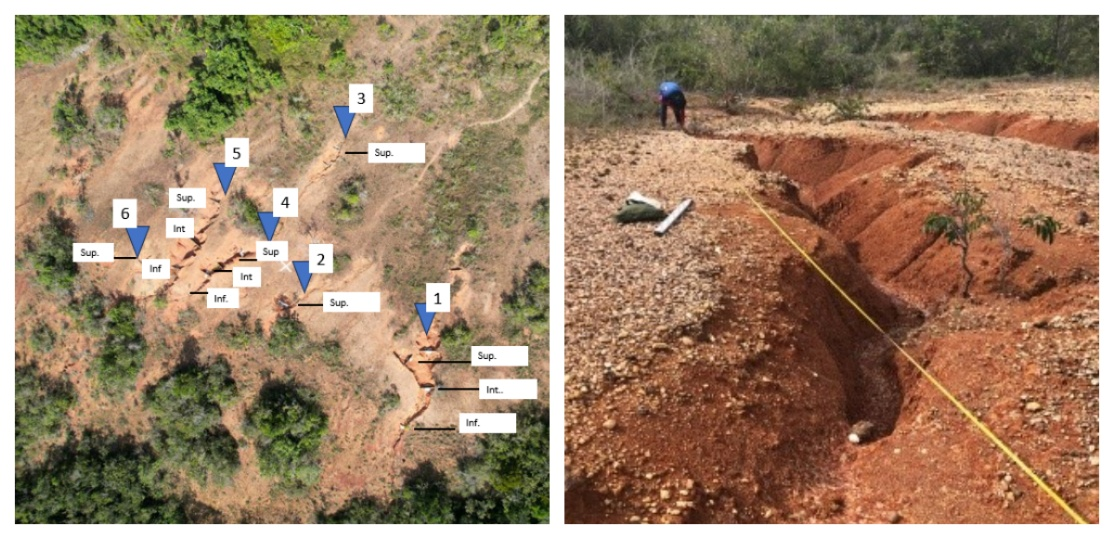
\includegraphics[width=0.9\linewidth,height=\textheight,keepaspectratio]{figuras/fig_00b_feicoes_drone_campo.jpeg}

}

\caption{\label{fig-feicoes-campo}Feições de erosão linear no sítio
experimental.}

\end{figure}%

\emph{Nota: Ortomosaico derivado de VANT mostrando a distribuição
espacial das feições erosivas mapeadas e medição em campo dos parâmetros
morfométricos (profundidade, largura e comprimento) em uma das feições
erosivas ativas.}

Todas as propriedades de entrada do Plintossolo foram obtidas de
medições em campo e análises laboratoriais conduzidas em amostras
coletadas no sítio experimental. A velocidade de infiltração básica
(VIB) foi determinada in situ por ensaios com infiltrômetro de duplo
anel em três horizontes representativos (Ap, BAc e Bf), resultando em
valores de 3,13, 1,53 e 1,59 cm/h, respectivamente, que confirmam que os
horizontes plíntico e subplíntico impõem impedância hidráulica abaixo do
limiar de referência adotado (\(VIB_{ref}\) = 6,0 cm/h). A saturação por
alumínio (\(m_{Al}\)) foi quantificada por análise de fertilidade de
rotina em amostras de cada horizonte genético, com valores variando de
15,2\% no Ap a 99,2\% no Bf, gradiente vertical consistente com a
lixiviação progressiva de bases e concentração de alumínio trocável em
profundidade.

Os parâmetros geotécnicos (coesão efetiva \(c\) = 13,02 kPa, ângulo de
atrito interno \(\phi\) = 34,93° e peso específico saturado
\(\gamma_{sat}\) = 19,93 kN/m³) foram determinados por ensaio de
cisalhamento direto (ASTM D3080) em amostras indeformadas extraídas do
horizonte Bt sob condições saturadas. A erodibilidade \(K_{RUSLE}\) =
0,035 t h MJ\(^{-1}\) mm\(^{-1}\) foi estimada a partir da distribuição
granulométrica, teor de matéria orgânica, código de estrutura e classe
de permeabilidade do horizonte superficial utilizando o nomograma padrão
\citep{wischmeier_et_al_1971}.

Dois perfis virtuais (Latossolo e Argissolo) foram parametrizados a
partir de valores medianos da literatura regional para VIB, saturação
por alumínio, propriedades geotécnicas e \(K_{RUSLE}\)
\citep{silva_et_al_2009, bertoni_lombardi_neto_2017}. O Latossolo opera
como controle negativo
(\(\alpha \approx \beta \approx \gamma \approx 1\)), representando solos
bem drenados sem impedância hidráulica, toxicidade ou feições erosivas
profundas, enquanto o Argissolo funciona como controle parcial,
compartilhando impedância hidráulica moderada no horizonte Bt, porém sem
plintita ou toxicidade extrema por alumínio. As propriedades dos três
perfis são sumarizadas na Tabela 3.

Tabela 3. Propriedades dos três perfis de solo utilizados no
experimento.

\begin{longtable}[]{@{}
  >{\raggedright\arraybackslash}p{(\linewidth - 6\tabcolsep) * \real{0.2500}}
  >{\raggedleft\arraybackslash}p{(\linewidth - 6\tabcolsep) * \real{0.2500}}
  >{\raggedleft\arraybackslash}p{(\linewidth - 6\tabcolsep) * \real{0.2500}}
  >{\raggedleft\arraybackslash}p{(\linewidth - 6\tabcolsep) * \real{0.2500}}@{}}
\toprule\noalign{}
\begin{minipage}[b]{\linewidth}\raggedright
Propriedade
\end{minipage} & \begin{minipage}[b]{\linewidth}\raggedleft
Plintossolo (campo)
\end{minipage} & \begin{minipage}[b]{\linewidth}\raggedleft
Latossolo (virtual)
\end{minipage} & \begin{minipage}[b]{\linewidth}\raggedleft
Argissolo (virtual)
\end{minipage} \\
\midrule\noalign{}
\endhead
\bottomrule\noalign{}
\endlastfoot
VIB superior (cm/h) & 3,13 & 12,0 & 4,5 \\
VIB intermediária (cm/h) & 1,53 & 9,0 & 2,5 \\
VIB inferior (cm/h) & 1,59 & 7,0 & 2,8 \\
\(m_{Al}\) Ap (\%) & 15,2 & 10,0 & 20,0 \\
\(m_{Al}\) subsuperfície (\%) & 84--99 & 20,0 & 45,0 \\
\(c\) (kPa, saturado) & 13,02 & 30,0 & 18,0 \\
\(\phi\) (°) & 34,93 & 30,0 & 32,0 \\
\(\gamma_{sat}\) (kN/m³) & 19,93 & 18,0 & 19,0 \\
\(H_c\) (m) & 3,35 & 5,77 & 4,33 \\
\(H/H_c\) médio & 0,28 & 0,00 & 0,08 \\
\(K_{RUSLE}\) (t h MJ\(^{-1}\) mm\(^{-1}\)) & 0,035 & 0,015 & 0,025 \\
\end{longtable}

\emph{Nota: Os valores do Plintossolo foram obtidos de medições em
campo; os valores do Latossolo e do Argissolo foram parametrizados a
partir da literatura regional.}

\subsection{4.2 Delineamento
multi-classe}\label{delineamento-multi-classe}

O experimento adota delineamento com fator fixo principal (classe de
solo, três níveis) e três parcelas de solo nu por sítio, dispostas ao
longo do gradiente de vertente no sítio-alvo (S1, 3 posições × 1
repetição) e agrupadas em posição única nos sítios-controle (S2 e S3, 1
posição × 3 repetições). A replicação temporal ao longo de dois anos
hidrológicos (dezenas de eventos erosivos por estação) compensa o número
reduzido de unidades espaciais, gerando centenas de observações
independentes de \(K_{obs}\) por sítio. Os três sítios experimentais
representam classes pedológicas com gradiente decrescente de
amplificação esperada para os termos \(\alpha\), \(\beta\) e \(\gamma\).

O sítio-alvo (S1) é instalado no Plintossolo Argilúvico Distrófico
descrito na seção 4.1, onde VIB varia de 3,13 cm/h no terço superior a
1,53 cm/h no intermediário, saturação por alumínio atinge 99,2\% no
horizonte BAc e seis feições erosivas com \(H/H_c\) de 0,12--0,45 foram
inventariadas. O sítio-controle negativo (S2) é instalado em Latossolo
Vermelho-Amarelo Distrófico, preferencialmente na mesma região
fisiográfica, selecionado por apresentar VIB tipicamente superior a 6
cm/h, saturação por alumínio inferior a 30\%, espessura homogênea do
horizonte Bw sem impedância hidráulica abrupta e ausência de feições
erosivas lineares ativas. O sítio-controle parcial (S3) é instalado em
Argissolo Vermelho-Amarelo Distrófico, com gradiente textural abrupto
(horizonte Bt adensado) que reproduz impedância hidráulica similar à do
Plintossolo, porém sem plintita e com saturação por alumínio
intermediária (tipicamente 30--60\%), constituindo classe que isola o
efeito do regime hidráulico (\(\alpha\)) das demais amplificações.

\subsection{4.3 Parcelas de erosão e distribuição por
sítio}\label{parcelas-de-erosuxe3o-e-distribuiuxe7uxe3o-por-suxedtio}

As parcelas seguem o padrão Wischmeier (\textcolor{red}{22,13 m de
comprimento na direção do declive × 1,83 m de largura = 40,5 m²}), com
\textcolor{red}{calhas coletoras (Geib) na extremidade inferior
conectadas a tanques de armazenamento de sedimentos}. Cada parcela é
delimitada por \textcolor{red}{chapas galvanizadas enterradas a 15 cm}
para evitar entrada lateral de escoamento. A superfície das parcelas
principais é mantida em pousio (solo nu e capinado) durante o período
experimental para isolar o fator \(K\) dos efeitos de \(C\) e \(P\)
(\(C = P = 1{,}0\)). A configuração da parcela individual e a
distribuição das 14 unidades nos três sítios são apresentadas na Fig.
Figura~\ref{fig-esquema}.

\begin{figure}

\centering{

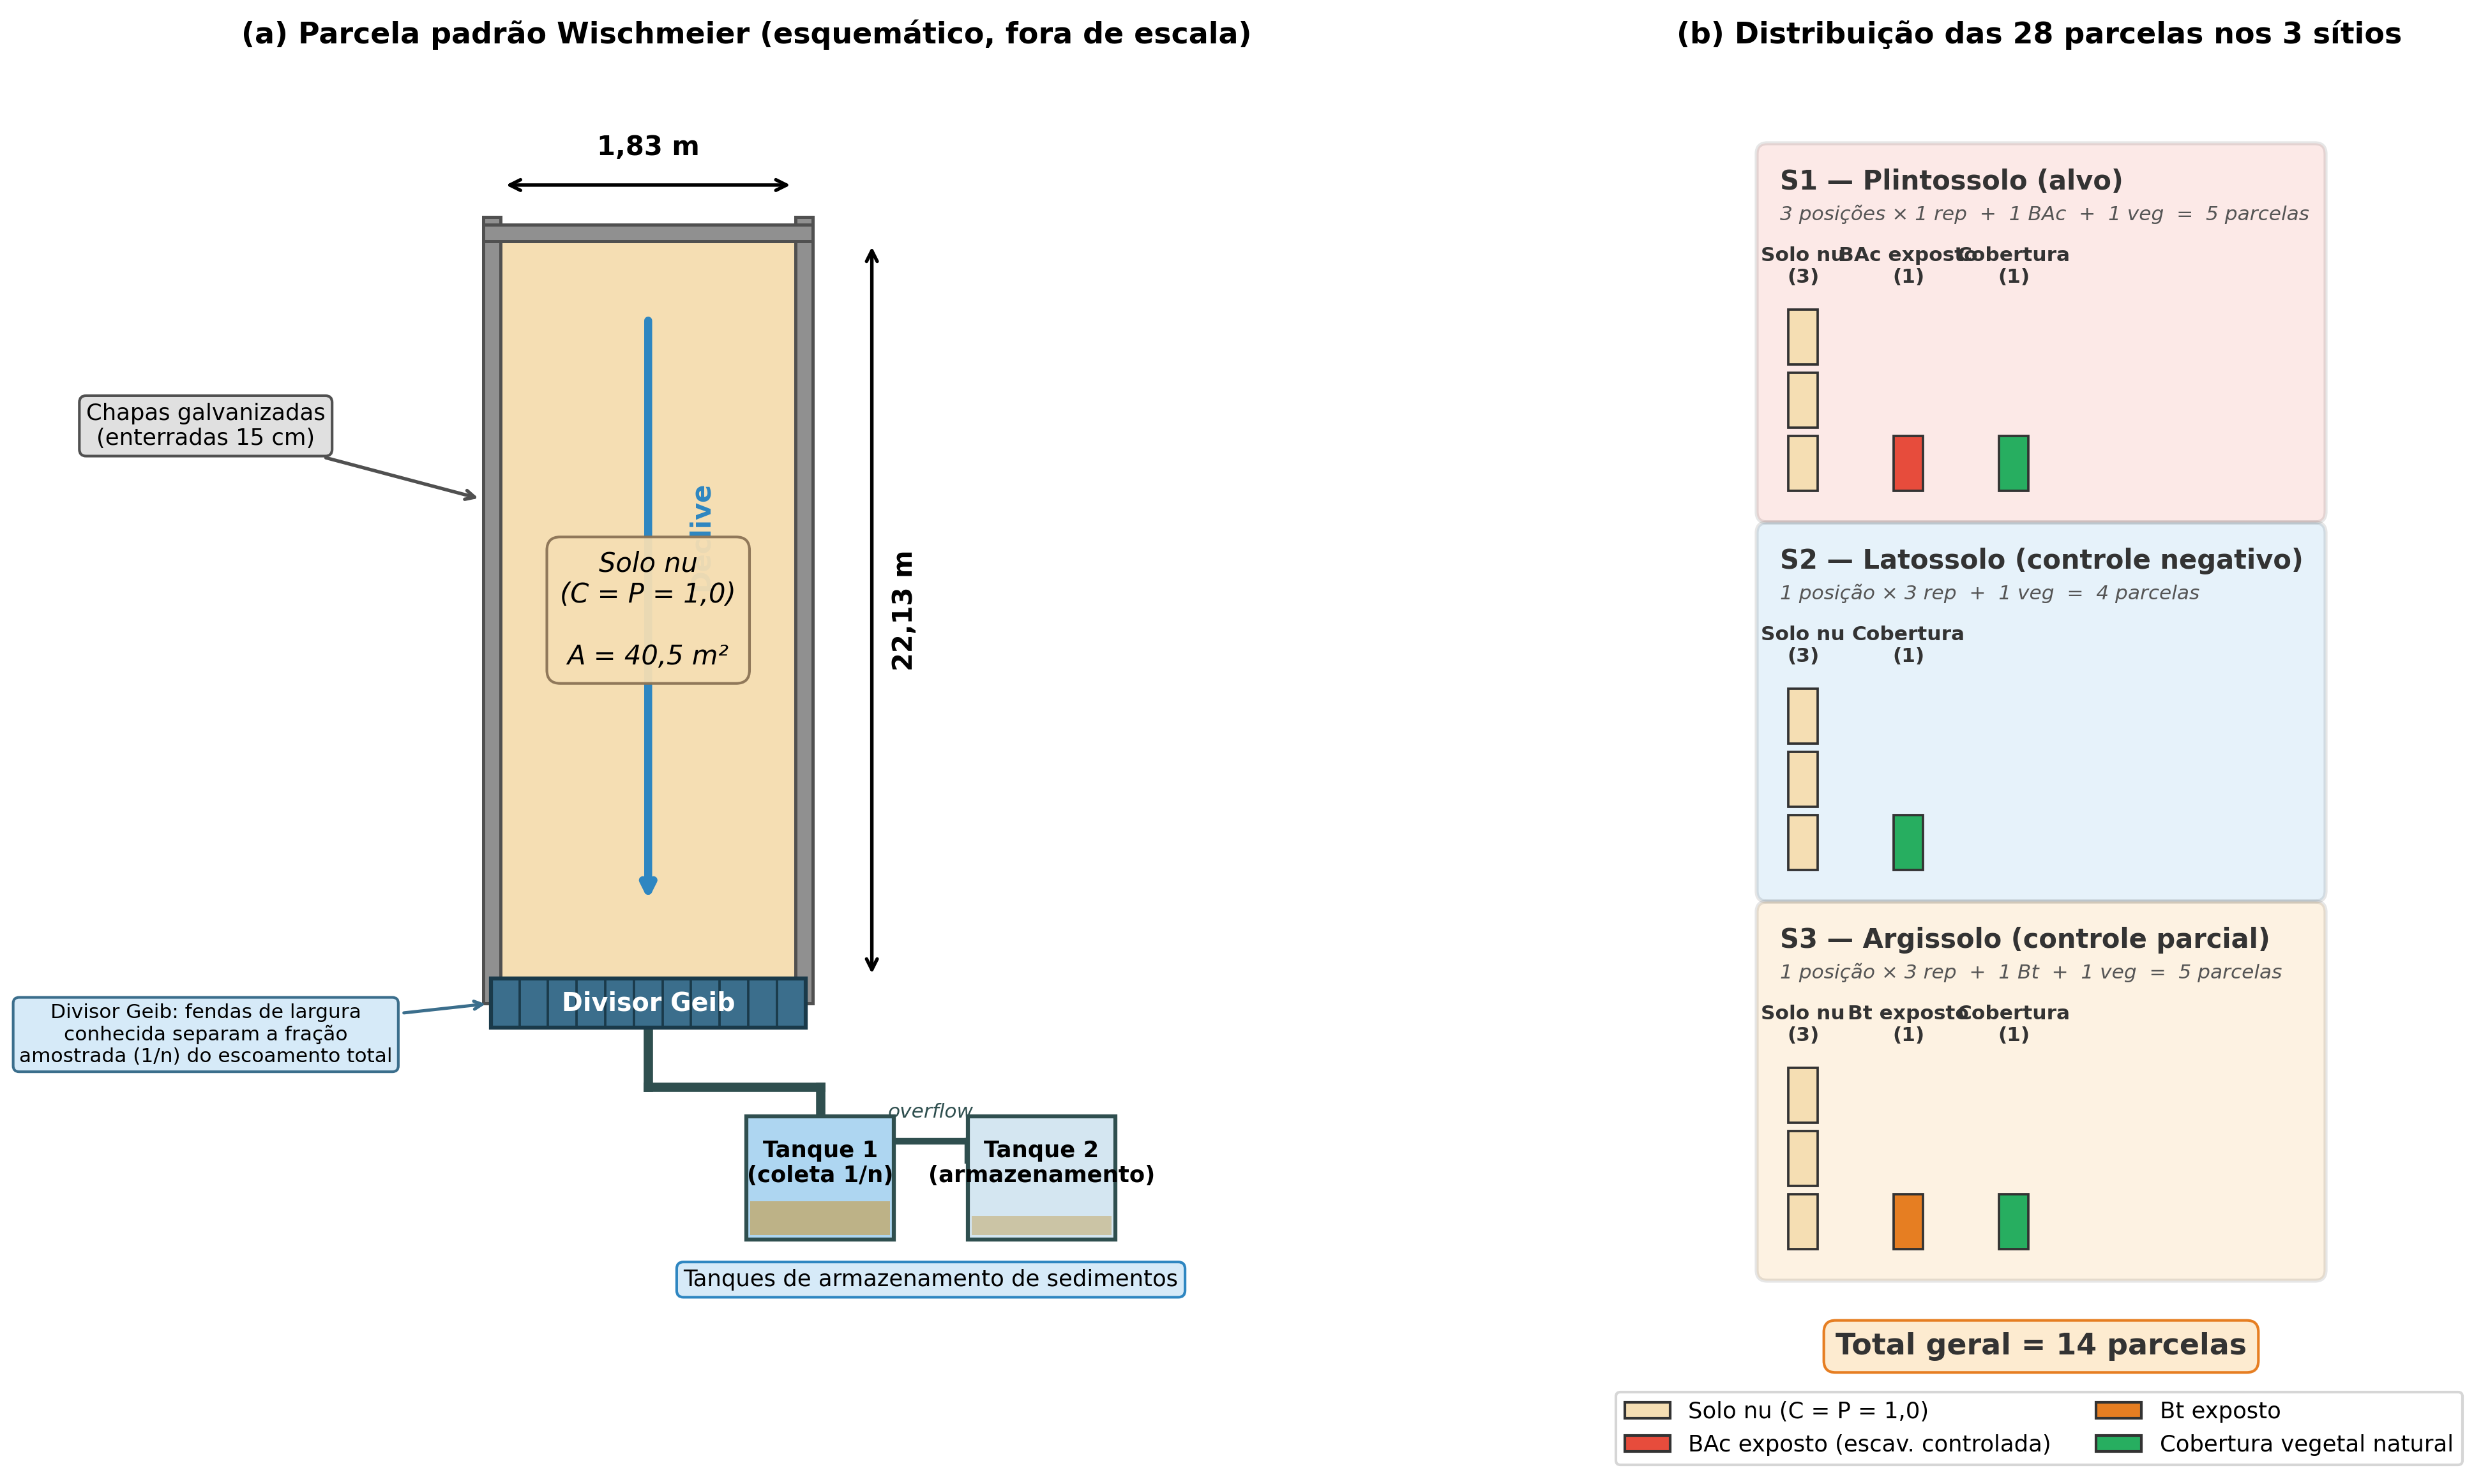
\includegraphics[width=1\linewidth,height=\textheight,keepaspectratio]{figuras/fig_esquema_parcela_experimento.png}

}

\caption{\label{fig-esquema}Esquema do experimento de erosão. (a)
Parcela padrão Wischmeier com divisor Geib, tanques de coleta e
armazenamento de sedimentos e chapas galvanizadas de delimitação
lateral. (b) Distribuição das parcelas nos três sítios pedológicos.}

\end{figure}%

A configuração física descrita na Fig. Figura~\ref{fig-esquema} reproduz
o desenho clássico de parcelas de monitoramento de erosão hídrica
empregado em condições edafoclimáticas brasileiras (Fig.
Figura~\ref{fig-geib}), em que o divisor Geib de múltiplas aberturas
fraciona o deflúvio excedente do primeiro tanque para o segundo,
ampliando a capacidade de coleta sem perda de representatividade
amostral \citep{melo_neto_et_al_2021}.

\begin{figure}

\begin{minipage}{0.50\linewidth}

\centering{

\pandocbounded{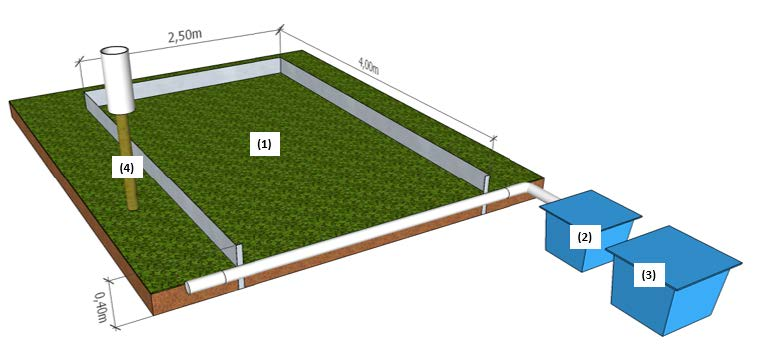
\includegraphics[keepaspectratio]{figuras/geib_a.jpeg}}

}

\subcaption{\label{fig-geib-a}Croqui da parcela com divisor Geib e
tanques de coleta}

\end{minipage}%
%
\begin{minipage}{0.50\linewidth}

\centering{

\pandocbounded{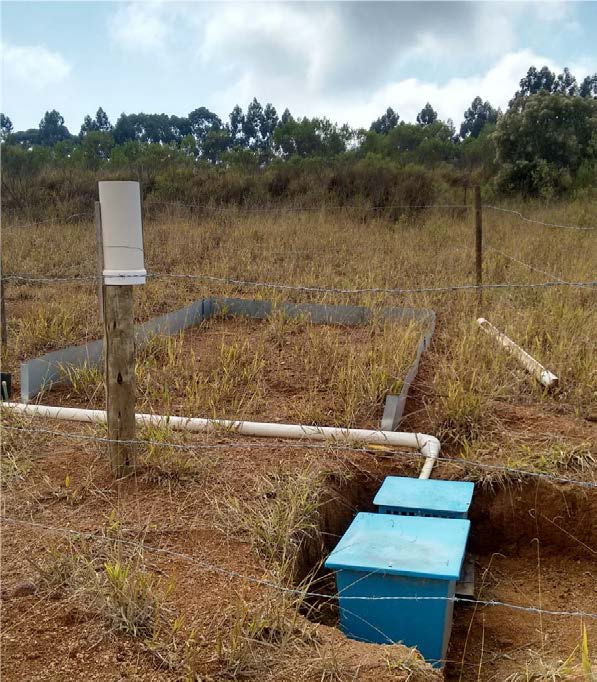
\includegraphics[keepaspectratio]{figuras/geib_b.jpeg}}

}

\subcaption{\label{fig-geib-b}Parcela instalada em campo}

\end{minipage}%

\caption{\label{fig-geib}Parcela de monitoramento de erosão hídrica do
solo com divisor Geib. (a) Croqui esquemático e (b) vista de campo.
Adaptado de \citet{melo_neto_et_al_2021} (CC BY 4.0).}

\end{figure}%

No sítio S1 (Plintossolo), o arranjo compreende \textcolor{red}{3
parcelas em solo nu (3 posições × 1 repetição, ao longo do gradiente de
VIB)}, \textcolor{red}{1 parcela com horizonte BAc exposto por escavação
controlada} para isolar o efeito de \(\beta\) e \textcolor{red}{1
parcela com cobertura vegetal natural} para quantificar a interação
\(\beta \times C\), totalizando \textcolor{red}{5 parcelas}. No sítio S2
(Latossolo), \textcolor{red}{3 parcelas em solo nu (1 posição × 3
repetições) e 1 parcela com cobertura vegetal} constituem o arranjo
mínimo necessário para estimar \(K_{obs}\) e verificar se
\(\delta \approx 1{,}0\) (\textcolor{red}{4 parcelas}). No sítio S3
(Argissolo), \textcolor{red}{3 parcelas em solo nu (1 posição × 3
repetições), 1 parcela com horizonte Bt exposto e 1 parcela com
cobertura vegetal} permitem isolar a contribuição do gradiente textural
(\textcolor{red}{5 parcelas}). \textcolor{red}{O total geral do
experimento é de 14 parcelas}.

\subsection{4.4 Protocolo de ensaios}\label{protocolo-de-ensaios}

\subsubsection{4.4.1 Ensaios comuns às três
classes}\label{ensaios-comuns-uxe0s-truxeas-classes}

O protocolo de monitoramento em campo compreende quatro componentes
simultâneos realizados durante \textcolor{red}{dois anos hidrológicos
consecutivos (abril a março)}, cobrindo a totalidade da estação chuvosa
(abril--agosto) e o período seco (setembro--março). A medição contínua
de precipitação utiliza \textcolor{red}{pluviógrafo de báscula
(resolução 0,2 mm, intervalo de registro de 5 min) instalado na crista
de cada vertente}, para cálculo do índice de erosividade \(R\)
(EI\(_{30}\)) por evento \citep{wischmeier_smith_1978}. A coleta de
sedimentos em \textcolor{red}{tanques de armazenamento} ocorre após cada
evento erosivo com precipitação superior a 10 mm, quantificando a perda
de solo por parcela em t ha\(^{-1}\) evento\(^{-1}\). A VIB é medida
sazonalmente por \textcolor{red}{infiltrômetro de anéis duplos (3
posições × 3 repetições por sítio)} e \textcolor{red}{amostras de solo
são coletadas para determinação de granulometria completa (com areia
muito fina separada), matéria orgânica (Walkley-Black ou combustão
seca), complexo sortivo completo (pH, Al³⁺, H+Al, CTC, V\%, saturação
por alumínio \(m\)), limites de Atterberg (LL, LP, IP), densidade do
solo e de partículas (\(\gamma_{sat}\)) e mineralogia por difração de
raios X (DRX) do horizonte diagnóstico}. Cada sítio conta com
\textcolor{red}{levantamento topográfico por estação total ou GNSS-RTK}
para determinação dos fatores \(L\) e \(S\).

\textcolor{red}{O ensaio de cisalhamento direto em condição saturada
(tensões normais de 25, 50, 100 e 200 kPa) é realizado em amostras
indeformadas do horizonte diagnóstico de cada classe} (Fig.
Figura~\ref{fig-sitio}), fornecendo coesão (\(c\)) e ângulo de atrito
(\(\phi\)) para cálculo de \(H_c\) pela Equação~\ref{eq-hc}.
\textcolor{red}{A condutividade hidráulica saturada por horizonte
(permeâmetro de carga constante) é determinada em amostras indeformadas
de dois a três horizontes por perfil}, validando a presença ou ausência
de impedância hidráulica abrupta.

\begin{figure}

\centering{

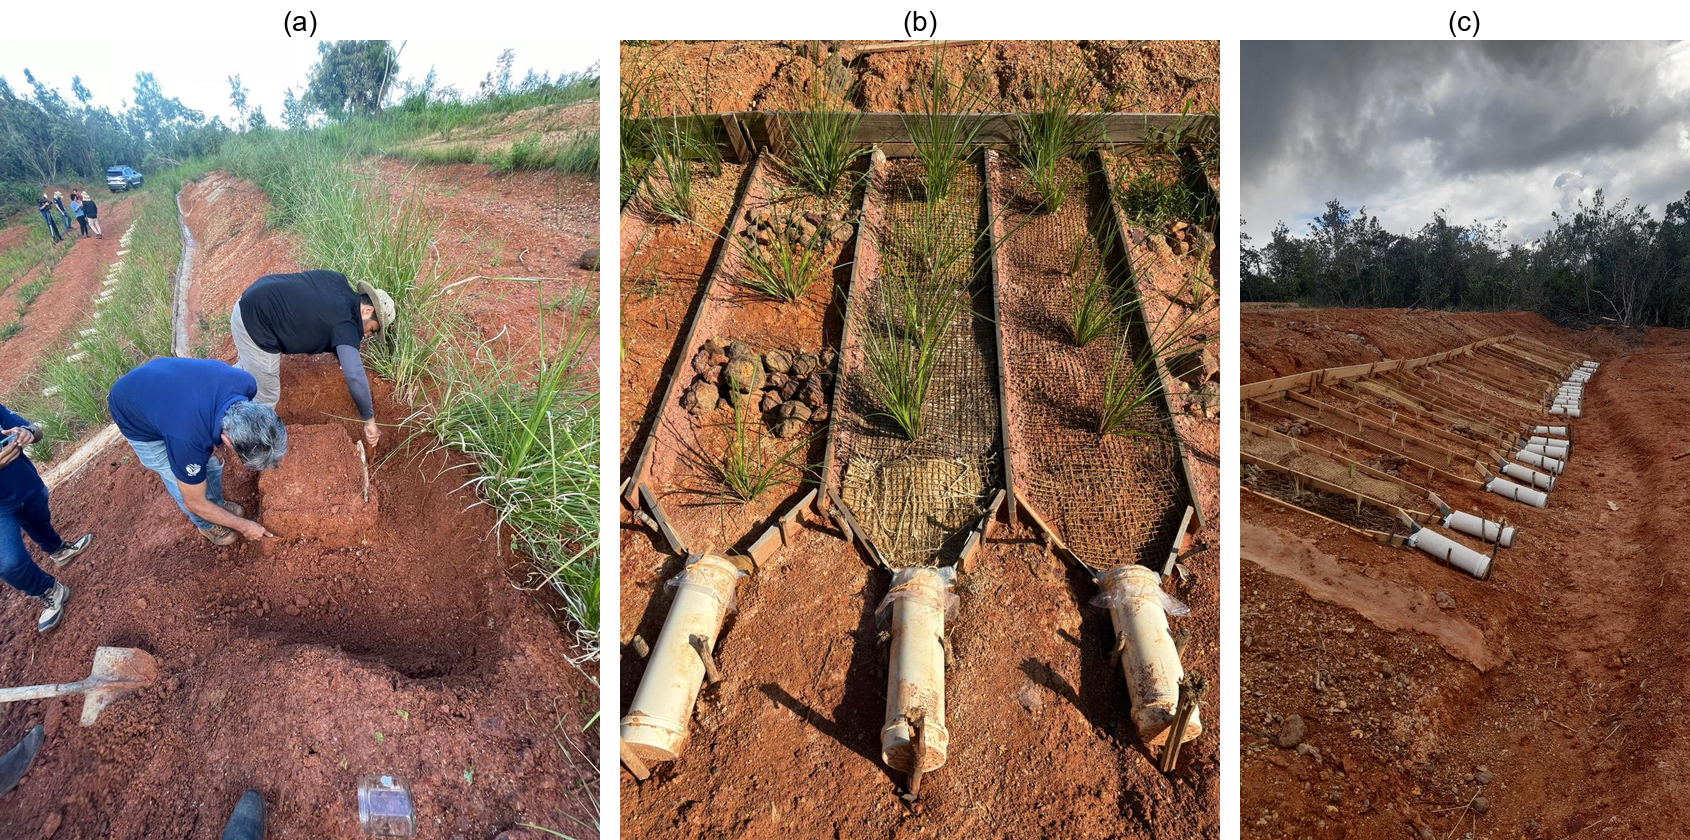
\includegraphics[width=1\linewidth,height=\textheight,keepaspectratio]{figuras/fig_09_sitio_experimental.png}

}

\caption{\label{fig-sitio}Elementos do sítio experimental em Plintossolo
Háplico, Tabuleiros Costeiros de Sergipe. (a) Bloco indeformado extraído
para ensaio de cisalhamento direto (\(c\) = 13,02 kPa, \(\phi\) =
34,93°). (b) Parcelas de coleta de sedimentos posicionadas na base do
talude erosivo. (c) Vista geral do talude com feições erosivas ativas.}

\end{figure}%

\subsubsection{4.4.2 Ensaios específicos por
classe}\label{ensaios-especuxedficos-por-classe}

No sítio S1 (Plintossolo), o monitoramento de profundidade das feições
adjacentes às parcelas utiliza \textcolor{red}{pinos de erosão (20 pinos
por feição, espaçamento de 1 m longitudinal × 0,5 m transversal,
leituras quinzenais)}, para quantificar o incremento volumétrico
atribuível a colapso de taludes e incisão vertical. A
\textcolor{red}{parcela com horizonte BAc exposto por escavação
controlada} permite isolar o efeito da toxicidade extrema (\(m\) =
99,2\%) sobre a erodibilidade observada. \textcolor{red}{Um inventário
completo das feições erosivas (profundidade, largura, comprimento,
\(H/H_c\)) é realizado semestralmente}.

No sítio S2 (Latossolo), não se preveem pinos de erosão nem parcelas com
horizonte exposto, dado que a hipótese H5 prediz
\(\delta \approx 1{,}0\) (ausência de amplificação). \textcolor{red}{A
mineralogia por DRX} confirma a presença de gibbsita e oxi-hidróxidos de
ferro responsáveis pela microagregação estável típica de Latossolos
\citep{silva_et_al_2009}.

No sítio S3 (Argissolo), \textcolor{red}{pinos de erosão são instalados
apenas se feições erosivas lineares forem identificadas durante o
inventário inicial}. \textcolor{red}{Uma parcela com horizonte Bt
exposto} permite avaliar se a impedância hidráulica do gradiente
textural abrupto, sem toxicidade extrema por alumínio, é suficiente para
gerar \(\alpha > 1\) isoladamente.

\subsection{\texorpdfstring{4.5 Cálculo de
\(K_{obs}\)}{4.5 Cálculo de K\_\{obs\}}}\label{cuxe1lculo-de-k_obs}

Para cada parcela em solo nu (\(C = P = 1\)), \(K_{obs}\) é obtido por
inversão da Equação~\ref{eq-usle} (Equação~\ref{eq-kobs}).

\begin{equation}\phantomsection\label{eq-kobs}{
K_{obs} = \dfrac{A_{obs}}{R \times L \times S}
}\end{equation}

onde \(A_{obs}\) é a perda de solo medida (t ha\(^{-1}\) ano\(^{-1}\)),
\(R\) a erosividade acumulada anual calculada a partir dos registros
pluviográficos, \(L\) o fator de comprimento calculado pela fórmula de
\citet{renard_et_al_1997} e \(S\) o fator de declividade medido por
estação total em cada parcela.

O fator \(K_{RUSLE}\) para o mesmo material é estimado pela
Equação~\ref{eq-nomograma} a partir dos dados de granulometria, matéria
orgânica e classificação de estrutura e permeabilidade do horizonte
exposto. A razão \(\delta = K_{obs}/K_{RUSLE}\) quantifica a
discrepância entre erodibilidade observada e prevista, que constitui a
variável-resposta do modelo de correção.

\subsection{4.6 Procedimento de
calibração}\label{procedimento-de-calibrauxe7uxe3o}

A calibração dos cinco parâmetros livres (\(n_1\), \(\beta_{max}\),
\(k_2\), \(k_3\), \(n_3\)) segue protocolo sequencial em quatro etapas,
tirando proveito da estrutura multi-classe para isolar cada termo.

A primeira etapa (verificação do controle negativo) compara
\(\delta_{S2}\) (Latossolo) com a unidade. Se
\(\delta_{S2} \approx 1{,}0\) (teste t unilateral, \(\alpha\) = 0,05),
confirma-se que a USLE é adequada para o Latossolo e que qualquer
discrepância observada nos demais sítios é atribuível às propriedades
específicas de cada classe. Se \(\delta_{S2}\) diferir
significativamente da unidade, os expoentes calibrados nos sítios S1 e
S3 devem ser interpretados como correções relativas ao Latossolo, e não
absolutas.

A segunda etapa (calibração marginal de \(\alpha\)) compara
\(\delta_{S3}\) (Argissolo, que apresenta \(\alpha > 1\) mas
\(\beta \approx 1\) e \(\gamma \approx 1\)) com \(\delta_{S2}\)
(Latossolo, \(\alpha \approx 1\)). A razão \(\delta_{S3}/\delta_{S2}\),
atribuível predominantemente a \(\alpha\), permite estimar \(n_1\) por
regressão não linear univariada contra \(VIB_{ref}/VIB_{local}\),
utilizando as 12 parcelas em solo nu do Argissolo que cobrem três níveis
de VIB.

A terceira etapa (calibração de \(\beta\)) utiliza as parcelas do sítio
S1 (Plintossolo) com horizonte Ap (\(m\) = 15,2\%) e horizonte BAc
exposto (\(m\) = 99,2\%), na mesma posição da vertente, controlando VIB.
A diferença de \(\delta\) entre horizontes, descontado o efeito de
\(\alpha\) já calibrado, é atribuída a \(\beta\), permitindo estimar
\(\beta_{max}\) e \(k_2\) por ajuste da sigmoide
(Equação~\ref{eq-beta}). Uma confirmação independente é possível
comparando as parcelas com Bt exposto no Argissolo (S3, \(m\)
intermediário) com as de BAc exposto no Plintossolo (S1, \(m\) extremo).

A quarta etapa (calibração de \(\gamma\)) utiliza as parcelas do sítio
S1 adjacentes a feições com \(H/H_c\) distinto (F2 com \(H/H_c\) = 0,12
vs.~F5 com \(H/H_c\) = 0,45). A perda total de solo (parcela + pinos de
erosão) fornece a base para isolar a contribuição de \(\gamma\), uma vez
que \(\alpha\) e \(\beta\) já foram calibrados. O resíduo
\(\delta_{residual} = \delta_{obs} / (\alpha \times \beta)\) é atribuído
a \(\gamma\), e os parâmetros \(k_3\) e \(n_3\) são estimados por
regressão não linear de \(\delta_{residual}\) contra \(H/H_c\).

A calibração final (simultânea) utiliza otimização por mínimos quadrados
não lineares (Levenberg-Marquardt) da Equação~\ref{eq-kplint-exp}
completa contra todos os valores de \(\delta_{obs}\) disponíveis nos
três sítios (n = 56 parcelas), partindo dos valores iniciais obtidos nas
etapas marginais. O intervalo de confiança dos parâmetros é estimado por
bootstrap paramétrico (1000 reamostras).

\subsection{4.7 Validação}\label{validauxe7uxe3o}

A estrutura multi-classe permite estratégia de validação em dois níveis.
A validação interna utiliza validação cruzada leave-one-out (LOOCV)
sobre as observações dos três sítios combinados. A validação cruzada
entre sítios (cross-site validation) calibra o modelo com dados de dois
sítios e testa no terceiro, repetindo para cada combinação, avaliando a
transferência do fator de correção entre classes pedológicas. A
validação externa, em fase posterior, requer aplicação do protocolo em
pelo menos um sítio adicional com Plintossolo de características
contrastantes, preferencialmente na Amazônia Oriental (Pará ou Maranhão)
ou nos Tabuleiros Costeiros da Bahia.

A avaliação de desempenho utiliza quatro métricas (Equações \ref{eq-r2}
a \ref{eq-pbias}).

\begin{equation}\phantomsection\label{eq-r2}{
R^2 = 1 - \dfrac{\sum(K_{obs,i} - K_{pred,i})^2}{\sum(K_{obs,i} - \bar{K}_{obs})^2}
}\end{equation}

\begin{equation}\phantomsection\label{eq-rmse}{
RMSE = \sqrt{\dfrac{1}{n}\sum_{i=1}^{n}(K_{obs,i} - K_{pred,i})^2}
}\end{equation}

\begin{equation}\phantomsection\label{eq-nse}{
NSE = 1 - \dfrac{\sum(K_{obs,i} - K_{pred,i})^2}{\sum(K_{obs,i} - \bar{K}_{obs})^2}
}\end{equation}

\begin{equation}\phantomsection\label{eq-pbias}{
PBIAS = \dfrac{\sum(K_{obs,i} - K_{pred,i})}{\sum K_{obs,i}} \times 100
}\end{equation}

Adicionalmente, o teste H4 (superioridade do modelo multiplicativo) é
avaliado por Critério de Informação de Akaike corrigido (AICc)
comparando quatro modelos candidatos: \(K_{RUSLE}\) isolado (sem
correção), modelo aditivo (\(K_{RUSLE} + \alpha + \beta + \gamma\)),
modelo multiplicativo parcial (apenas \(\alpha\)) e modelo
multiplicativo completo (Equação~\ref{eq-kplint-exp}). O teste H5
(especificidade pedológica) é avaliado por ANOVA de \(\delta\) entre as
três classes de solo, seguida de contrastes ortogonais (Plintossolo
vs.~Latossolo, Plintossolo vs.~Argissolo, Argissolo vs.~Latossolo).

\section{5. Pressupostos e
limitações}\label{pressupostos-e-limitauxe7uxf5es}

A proposta fundamenta-se em seis pressupostos cuja violação pode
comprometer a calibração. O primeiro pressupõe que a variação de VIB ao
longo da vertente é estável entre eventos e estações, o que pode não se
verificar sob compactação progressiva ou recuperação estrutural sazonal;
o monitoramento sazonal de VIB (seção 4.4) permite avaliar essa
premissa. O segundo pressupõe que a saturação por alumínio do horizonte
diagnóstico é o principal determinante da supressão de cobertura
vegetal, isolando o efeito de \(\beta\) do fator \(C\); em sítios onde
outros fatores (sombreamento, tráfego animal) controlam a cobertura, a
separação entre \(\beta\) e \(C\) torna-se ambígua.

O terceiro pressuposto é que o colapso de taludes capturado pelo fator
\(\gamma\) ocorre dentro ou adjacente à parcela de erosão; se o colapso
mobiliza material a montante da parcela, a perda medida subestima a
contribuição geotécnica. O quarto é a independência entre os três
fatores de correção (multiplicatividade), premissa que pode ser violada
se, por exemplo, a redução de VIB for causada pela mesma compactação que
altera a coesão. O quinto pressupõe que dois anos hidrológicos capturam
variabilidade climática suficiente para calibração robusta, premissa
dependente da ocorrência de eventos extremos no período amostral. O
sexto pressupõe que os três sítios experimentais estão submetidos a
regime erosivo comparável (mesma zona climática, faixa de declividade
similar), de modo que as diferenças de \(\delta\) entre classes sejam
atribuíveis às propriedades do solo e não a covariáveis externas; a
seleção de sítios na mesma região fisiográfica (Tabuleiros Costeiros)
mitiga esse risco.

O desenho multi-classe elimina a principal limitação do estudo original
(n = 1 para calibração) ao expandir a base de observações para 56
parcelas em três classes contrastantes, permitindo validação cruzada
entre sítios. A proposta permanece restrita à faixa dos Tabuleiros
Costeiros do Nordeste brasileiro, e a generalização dos expoentes
calibrados para outras unidades fisiográficas (Amazônia Oriental,
Cerrado) requer campanha posterior.

\section{6. Resultados esperados e
contribuição}\label{resultados-esperados-e-contribuiuxe7uxe3o}

Com base nos dados de campo e na literatura, os seguintes resultados são
esperados por classe de solo. No sítio S2 (Latossolo), a erodibilidade
observada pode situar-se próxima à prevista pelo nomograma
(\(\delta \approx 1{,}0\)), confirmando que a microagregação estável por
oxi-hidróxidos compensa parcialmente a elevação de \(M\) pela
granulometria argilosa \citep{silva_et_al_2009}. No sítio S3
(Argissolo), o gradiente textural abrupto pode gerar amplificação
moderada (\(\delta \approx 1{,}5\)--2,0), atribuível predominantemente
ao fator \(\alpha\) sob VIB reduzida pela impedância do horizonte Bt,
com contribuição limitada de \(\beta\) e \(\gamma\). No sítio S1
(Plintossolo), a erodibilidade observada no terço intermediário (VIB =
1,53 cm/h) pode exceder a prevista pelo nomograma em fator de 2 a 4,
indicando subestimativa sistemática do \(K\) em regime de escoamento
hortoniano com toxicidade extrema.

O expoente \(n_1\) situa-se provavelmente na faixa 0,5--1,5, com valores
mais elevados correspondendo a maior sensibilidade do sistema à VIB. O
fator \(\beta_{max}\) é esperado na faixa 1,5--3,0, refletindo a
amplificação pela supressão de cobertura em horizontes com toxicidade
extrema por alumínio. O parâmetro \(k_3\) do fator geotécnico é o mais
incerto, pois depende da frequência e magnitude dos colapsos de talude
durante o período experimental, sendo esperados valores baixos (\(k_3\)
= 1--3) se os colapsos forem episódicos e elevados (\(k_3\) = 5--10) se
a estação chuvosa desencadear múltiplos eventos de ruptura.

A contribuição principal é metodológica, estabelecendo um protocolo
multi-classe replicável para quantificar a discrepância entre
\(K_{RUSLE}\) e erodibilidade efetiva em solos tropicais com erosão
linear, com validação cruzada entre classes pedológicas e identificação
de quais dos três mecanismos (regime hidráulico, toxicidade, geotécnica)
contribuem de modo preponderante para essa discrepância. A secundária é
operacional, oferecendo aos gestores de áreas degradadas um fator de
correção que pode ser aplicado com dados de campo rotineiros (VIB,
análise de solo, profundidade de feição) para melhorar a estimativa de
perda de solo em vertentes onde a USLE convencional subestima a erosão.

\section{Referências}\label{referuxeancias}

\renewcommand{\bibsection}{}
\bibliography{../referencias_artigos.bib}





\end{document}
